%-----------------------------------------------------------------------
\subsection{Receive Track Data}
%-----------------------------------------------------------------------
%\tbc
%Bernd Hekele

The block ``Receive Track Data'' is responsible for receiving Eurobalise-telegrams and Euroradio-messages from the API and perform several consistency checks on the input.

The block collects the telegrams of balises in order to build balise group messages. Euroradio messages are always delivered as a whole message. 

On each message, a consistency check is performed, before the data is validated according to the driving direction of the train. In general, messages not designated for the current driving direction of the train are not forwarded to the further processing.

After applying consistency checks, the data direction is validated.

Information of the odometer is used to control for the train leaving the expectation window of the balises. % TODO makes not much sense here.

\begin{figure}[H]
 \centering
 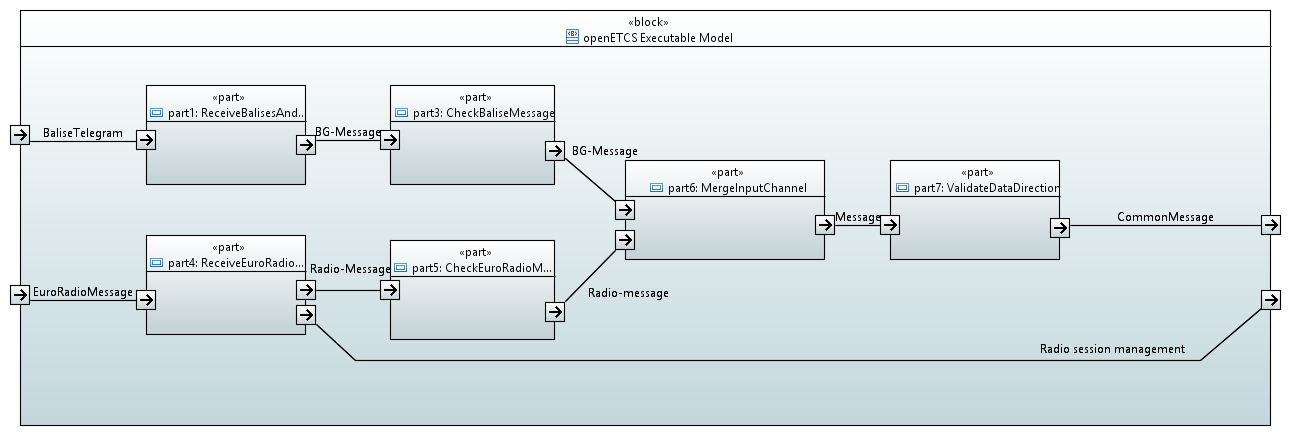
\includegraphics[width=\textwidth]{./images/Input-Messages4.PNG}
 % Input-Messages4.PNG: 0x0 pixel, 0dpi, nanxnan cm, bb=
 \caption{Structure of the Receive message and check consistency module}
 \label{fig:receiveAndCheckConsistencyArch}
\end{figure}


\subsubsection{Input}
For providing the output, the module needs different input data flows. An overview is provided in table \ref{tbl:ReceiveMessageAndCheckConsistencyInput}

\begin{table}[H]
  \begin{tabular}{| c | l | l | l | l |}
    \hline
    \textbf{Index} & \textbf{Input name} & \textbf{Input type} & \textbf{Source}\\ \hline
    0 & \texttt{apiRtmMessage} & \texttt{apiRtmMessage\_T} & API \\
    1 & \texttt{apiBaliseTelegram} & \texttt{API\_Telegram\_T} & API\\
    2 & \texttt{apiRadioDevice} & \texttt{int} & API\\
    3 & \texttt{connectionStatus} & \texttt{sessionStatus\_Type} & MoRC\\
    4 & \texttt{lastRelevantEventTimestamp} & \texttt{T\_internal\_Type} & MoRC or Database (?)\\
    5 & \texttt{tNvContact} & \texttt{T\_internal\_Type} & Database\\
    6 & \texttt{currentOdometry} & \texttt{odometry\_T} & Odometry\\
    7 & \texttt{lrbg} & \texttt{positionedBG\_T} & Database\\
    8 & \texttt{reset} & \texttt{bool} & internal\\
    \hline
  \end{tabular} 
  \caption{Overview over input}
  \label{tbl:ReceiveMessageAndCheckConsistencyInput}
\end{table}

\paragraph{Input 0: \texttt{apiRtmMessage}}

The Euroradio-/Eurobalise-message is originated from the openETCS-API. The API is described in the section \ref{chp_openETCS_API}.

In the current implementation, only messages with normal priority are used in the system. Emergency messages will not be processed.

%The type \texttt{RTM\_IN\_MESSAGE\_T}  is used for normal messages, which can contain connection confirmations, information about connection problems or data.
%\begin{table}[H]
%	\begin{tabular}{| c | l | l | l |}
%	 \hline
%	 \textbf{Index} & \textbf{Element name} & \textbf{Element type} & \textbf{Description}\\ \hline
%	 0 & RADIO\_DEVICE & ETCS\_ID\_T & Source interface of the message\\
%	 1 & REASON & RTM\_DIAGNOSTIC\_CODE\_T & Diagnostic code for connection problems\\
%	 2 & DATA & RTM\_MESSAGE\_T & Decoded message, CRC-checked\\
%	 \hline
%	\end{tabular}
%\end{table}

The input not only transfers the radio message but also information, if a message is present and if this message was decoded correctly and passed the lowlevel checks performed by the API.

The radio message itself consists of a header and a payload-part. The header part contains all variables of the message. The payload-part consists of all packets in the message.

\paragraph{Input 1: \texttt{apiBaliseTelegram}}

The telegram is build from 
\begin{itemize}
\item a present flag (bool)\\
Indicates the input decoded telegram parameter is “present”, i.e., the input has been updated by the API.
Only if the telegram is present the position information (incenterOfBalise) is to be used.\\
\item the decoded telegram including optional packets received from the balise.
\item the centerOfBalisePosition parameter. This parameter is used to give the position where the BTM has recognised the center of the balise telegram.
\end{itemize}

\paragraph{Input 2: \texttt{apiRadioDevice}}
The RTM-module may include multiple radio devices. When a handover between two RBCs is performed, messages can be received from both radio devices. The API provides information about the device, which received the message.

The values transmitted have to be defined by the API.

\paragraph{Input 3: \texttt{connectionStatus}}
The input \texttt{connectionStatus} will give information about the radio connection. This input is delivered by the session management module, not from the API. The information is needed to perform the timing check, which is depending on the connection state.

\begin{table}[H]
  \begin{tabular}{| l | p{9cm} |}
    \hline
    \textbf{Value} & \textbf{Interpretation}\\ \hline
    DISCONNECTED & The OBU is currently not connected to a RBC.\\
    CONNECTING & The OBU is currently connecting to the RBC. Received messages belong to the process of establishing a connection.\\
    CONNECTION\_ESTABLISHED &  The connection to RBC is established.\\
    \hline
  \end{tabular} 
  \caption{Possible values for the input \texttt{connectionStatus}}
  \label{tbl:connectionStatus}
\end{table}

% \paragraph{Input 4: \texttt{apiConsistencyError}}
% If the API detects a consistency error in the transmitted message, this error is reported to the model by the input \texttt{apiConsistencyError}.
% 
% Possible errors detectable by the API are:
% \begin{itemize}
%  \item CRC-error
%  \item Value range of variable exceeded
% \end{itemize}
% 
% 
% \begin{table}[H]
%   \begin{tabular}{| l | p{9cm} |}
%     \hline
%     \textbf{Value} & \textbf{Interpretation}\\ \hline
%     true & The API detected a consistency error.\\
%     false & No consistency error was detected by the API.\\
%     \hline
%   \end{tabular} 
%   \caption{Possible values for the input \texttt{apiConsistencyError}}
%   \label{tbl:apiConsistencyError}
% \end{table}

\paragraph{Input 4: \texttt{lastRelevantEventTimestamp}}

For monitoring the safe radio connection, it's necessary, that the time between two packets is less than the value of \texttt{T\_NVCONTACT}.

In situations like level-changes or announced radioholes, not the timestamp of the last message is relevant for comparison, but the timestamp of the last relevant event. This can be e.g. the timestamp of the level change or the timestamp of the timestamp of the moment, when the train was passing the end of the radiohole. 

For performing this check, the timestamp of the last relevant event is provided to the model as an \texttt{T\_internal\_Type}-type.

\paragraph{Input 5: \texttt{tNvContact}}

For monitoring the safe radio connection, the national value \texttt{T\_NVCONTACT} is needed as an input.

\paragraph{Input 6: \texttt{currentOdometry}}
Current information giving the odometry of the train. 

\paragraph{Input 7: \texttt{lrbg}}
The Last Relevant Balise Group. The information has been collected before by the train position function.

\paragraph{Input 8: \texttt{reset}}
To delete all data stored in the module (e.g. collected balise-telegrams, which do not yet form a complete message), a reset input can be used. If the input is set to \texttt{true}, all data kept in the module is deleted and no input is accepted.

\begin{table}[H]
  \begin{tabular}{| l | p{9cm} |}
    \hline
    \textbf{Value} & \textbf{Interpretation}\\ \hline
    true & All data kept in the module is deleted and no input is accepted.\\
    false & No action. Data at input is accepted.\\
    \hline
  \end{tabular} 
  \caption{Possible values for the input \texttt{reset}}
  \label{tbl:reset}
\end{table}

% A Eurobalise telegram consists of several fields shown in the table below. The table is an excerpt from the SRS, chapter 8.4.2.1. In this chapter the description of the fields can be found.
%  
%  
%  \begin{tabular}{| c | l | c  |}
%   \hline
%   \textbf{Field No.} & \textbf{VARIABLE} & \textbf{Length (bits)} \\ \hline
%   1 & Q\_UPDOWN & 1\\
%   2 & M\_VERSION & 7\\
%   3 & Q\_MEDIA & 1\\
%   4 & N\_PIG & 3\\
%   5 & N\_TOTAL & 3\\
%   6 & M\_DUP & 2\\
%   7 & M\_MCOUNT & 8\\
%   8 & NID\_C & 10\\
%   9 & NID\_BG & 14\\
%   10 & Q\_LINK & 1\\
%   \textit{-} & \textit{Packet 0 (Virtual balise cover) (optional)} & \textit{14}\\
%   \textit{-} & Information & variable\\
%   \textit{-} & Packet 255 & 8\\  
%   \hline
%  \end{tabular}
%  
%  \textbf{Relevant messages for track Utrecht-Amsterdam:} packets from balises: 3, 41, 42, 45, 46, 65, 72, 137, 255
%  
 


% \begin{itemize}
%  \item packets from balises: 3, 41, 42, 45, 46, 65, 72, 137, 255
% \end{itemize}
% \item unchecked Euroradio message
% \begin{itemize}
%  \item messages from rbc: 2, 3, 6, 8, 15, 24, 27, 32, 39, 41
%  \item packets from rbc: 3, 5, 15, 21, 27, 41, 42, 57, 58, 65, 68, 72, 80
% \end{itemize}
%\end{itemize}


\subsubsection{Output}
The output of the module provides the received and processed Euroradio and Eurobalise messages. The module combines messages both from Eurobalises and from Euroradio to one common dataflow.

Additionally, status information is provided. The status information consists of the following data:
\begin{itemize}
	\item Information, if the message has to be rejected in case of a consistency error, includeing further information about the error.
	\item Information, if an acknowledgement has to be sent to the RBC for the message
	\item Information about the radio connection. None or one of the following notifications:
	\begin{itemize}
		\item Confirmation for establishing a connection or reconnection
		\item Notification, that a established connection was lost, including the origin of the failure
		\item Notification, that a connection could not be (re)established after 3 attempts, includeing the origin of the failure
		\item Notification, that a connection could not be re-established after 3 attempts, includeing the origin of the failure
	\end{itemize}
\end{itemize}

An overview over the output dataflows is provided in table \ref{tbl:ReceiveMessageAndCheckConsistencyOutput}.

\begin{table}[H]
  \begin{tabular}{| c | l | l | l |}
    \hline
    \textbf{Index} & \textbf{Output name} & \textbf{Output type}\\ \hline
    0 & \texttt{present} & \texttt{bool}\\
    1 & \texttt{rejectionReason} & Boolean-Array (to be defined)\\
    2 & \texttt{acknowledgementRequired} & \texttt{bool}\\
    3 & \texttt{radioConnectionStatusFromAPI} & \texttt{RadioConnectionStatusFromAPI\_T}\\
    4 & \texttt{radioDeviceOut} & \texttt{int}\\
    5 & \texttt{applyServiceBreak} & \texttt{bool} \\
    6 & \texttt{badBaliseMessageToDMI} & \texttt{bool} \\
    7 & \texttt{receivedMessage} & \texttt{ReceivedMessage\_T} \\
    \hline
  \end{tabular} 
  \caption{Dataflow at output}
  \label{tbl:ReceiveMessageAndCheckConsistencyOutput}
\end{table}

\subparagraph{Output 0: \texttt{present}}
The present-flag specifies, if the data provided by the output \texttt{receivedMessage} is to be considered as present by the following modules or if it has to be ignored due to no new input data.

\begin{table}[H]
  \begin{tabular}{| l | p{13cm} |}
    \hline
    \textbf{Value} & \textbf{Interpretation}\\ \hline
    false & The data in this element is not present and has to be ignored. \\
    true & The data in this element is present and has to be processed by the following models. \\
    \hline
  \end{tabular} 
  \caption{Possible values for the output \texttt{present}}
  \label{tbl:rcvpresent}
\end{table}

\subparagraph{Output 1: \texttt{rejectedReason}}
In case of an inconsistent message, the output \texttt{rejectedReason} is giving information to the system, which problem occured. This information also has to be sent to the RBC as an error report by the responsible module.

\subparagraph{Output 2: \texttt{acknowledgementRequired}}

The \texttt{acknowledgementRequired}-dataflow indicates, whether the reception of the message has to be acknowledged to the RBC.

\begin{table}[H]
  \begin{tabular}{| l | p{13cm} |}
    \hline
    \textbf{Value} & \textbf{Interpretation}\\ \hline
    true & An acknowledgement has to be sent to the RBC for the current message delivered at output \texttt{receivedMessage} \\
    false & No acknowledgement has to be sent for the current message delivered at output \texttt{receivedMessage} \\
    \hline
  \end{tabular} 
  \caption{Possible values for the output \texttt{AcknowledgementRequired}}
  \label{tbl:AcknowledgementRequiredTable}
\end{table}

\subparagraph{Output 3: \texttt{radioConnectionStatusFromAPI}}
The output \texttt{radioConnectionStatusFromAPI} is used, when the RTM reports problems with the radio connection. The output is derived from the Alstom-API. %\textbf{TODO!} 
The output can be one of the following values:

\begin{table}[H]
  \begin{tabular}{| l | p{9cm} |}
    \hline
    \textbf{Value} & \textbf{Interpretation}\\ \hline
    CONNECTION\_CONFIRMATION & Confirmation for establishing a connection or reconnection\\
    CONNECTION\_LOST & Notification, that a established connection was lost\\
    CONNECTION\_FAILURE & Notification, that a connection could not be (re-)established after 3 attempts, includeing the origin of the failure\\
    
    CONNECTION\_NOT\_ESTABLISHED &  Notification, that a connection could not be re-established after 3 attempts, includeing the origin of the failure\\
    \hline
  \end{tabular} 
  \caption{Possible values for the output \texttt{radioConnectionStatusFromAPI}}
  \label{tbl:ConnectionStatusOutput}
\end{table}

\subparagraph{Output 4: \texttt{radioDeviceOut}}
The output radio device will give information, which device received a radio message. Trains equipped with two or more radio devices may receive messages on two interfaces in situations of a RBC handover.

\subparagraph{Output 5: \texttt{applyServiceBreak}}
The flag indicates the balise group the train just passed could not be processed correctly. The check results in the request for a service break.

\subparagraph{Output 6: \texttt{badBaliseMessageToDMI}}
Information to be passed to the DMI to indicate the reception of a ``bad balise'' to the driver.

\subparagraph{Output 7: \texttt{receivedMessage}}
The element \texttt{receivedMessage} consists of the type \texttt{ReceivedMessage\_T} combines both balise and radio messages to one common datatype. This datatype contains all variables and packets, which are possible for the given scenario.

\begin{table}[H]
  \begin{tabular}{| l | l | p{5.5cm} |}
  \hline
  \textbf{Name} & \textbf{Datatype} & \textbf{Description}\\ \hline
  \texttt{source} & Enumeration & Defines, if this is a Euroradio or Eurobalise message.\\
  \texttt{valid} & \texttt{bool} & true, if no consistency errors were detected.\\
  \texttt{metadata} & \texttt{Metadata\_T} & contains the metadata of the packets\\
  \texttt{BG\_Common\_Header} & \texttt{BG\_Header\_T} & Header of Eurobalise message\\
  \texttt{Radio\_Common\_Header} & \texttt{Radio\_TrackTrain\_Header\_T} & Header of Euroradio message\\
  \texttt{Packets} & structure of possible packets & -\\
  \hline
\end{tabular}
  \caption{Structure of \texttt{ReceivedMessage\_T}}
  \label{tbl:receivedMessage_structure}
\end{table}

The Eurobalise-common-header \texttt{BG\_Header\_T} consists of the fields visible in the SCADE-declaration. The structure corresponds to the structure defined in the SRS chapter 8.4.2.1. Some fields were removed since they are not needed anymore for further processing after building messages from separate telegrams.

The Euroradio-common-header \texttt{Radio\_TrackTrain\_Header\_T} consists of the fields visible in the SCADE declaration. The structure corresponds to the structure defined in the SRS chapter 8.4.4.6.1. The structure contains all variables required by possible \texttt{NID\_MESSAGE} values for the given scenario.

%\textbf{TODO:} Different definition of Radio-header than in SCADE!

%\textbf{TODO:} Note on packet type definitions and implementation details (which values were not used).

\textbf{Note:} Packet 44 not used (applications outside the ERTMS/ETCS system are not supported by this implementation).

%\textbf{TODO:} Define packets 136, 12 in SCADE.


\subsubsection{Macrofunction ReceiveBaliseAndBuildBG in Receive Track Data}%Mainfunction receive track data. Name should be be defined and substituded by the designer of the function. 
\paragraph{Reference to the SRS (or other requirements)}
\begin{itemize}
  \item Definition of the Balise Telegram: subset 26 section 7 and 8
  \item Interface to the BTM: Subset 36, section  4.2.2, 4.2.4, 4.2.9
  \item Handling of Balise Telegrams: Subset 26, sections 3.4.1 - 3.4.3, 3.16.2
  \item Check of the balise group Subset 26, section 3.16.2
  \item Determining the Orientation: 3.4.2
  \item Active Functions Table: 4.5.2
\end{itemize}
\paragraph{Short description of the functionality}
This function defines the interface of the OBU model to the openETCS generic API for Eurobalise Messages. On the interface, either a valid telegram is provided or a telegram is indicated which could not be received correct when passing the balise. The function passes the telegram without major changes of the information to the next entity for collecting the balise group information. This entity collects telegrams received via the interface into Balise Group Information.

\paragraph{Interface}
\paragraph{Functional Design Description}
\textbf{Design Constraints and Choices}
\begin{enumerate}
\item The decoding of balises is done at the API. Also, packets received via the interface are already transformed into a usable shape.
\item Only packets used inside the current model are passed via the interface:\\
Packet 5: Linking Information.\\
Linking Information is added to the linking array starting from index 0 without gaps. Used elements are marked as valid. Elements are sorted according to the order given by the telegram sequence.
\item Telegrams received as invalid are passed to the ``Check-Function'' to process errors in communication with the track side according to the requirements and in a single place.
Telegrams are added to the telegram array starting from index 0 without gaps. Used elements are marked as valid. Elements are stored according to the order given by the telegram sequence.
\item This function does not process information from the packets. The information is passed to the check without further processing of the values. 
\end{enumerate}

\paragraph{Reference to the Scade Model}
\textbf{only in special case or link to the Scade model}

\subsubsection{Macrofunction Check BG Consistency in Receive Track Data}%Mainfunction receive track data. Name should be be defined and substituded by the designer of the function. 
\paragraph{Reference to the SRS or other Requirements (or other requirements)}
\begin{itemize}
  \item Definition of the Balise Telegram: subset 26 section 7 and 8
  \item Handling of Balise Telegrams: Subset 26, sections 3.4.1 - 3.4.3, 3.16.2
  \item Check of the balise group Subset 26, section 3.16.2
  \item Active Functions Table: 4.5.2
\end{itemize}
\paragraph{Short description of the functionality}
This function has the task  to verify the completeness and correctness of the received messages from balis-groups.\\
A message consists of at least a telegram and a maximum of 8 telegrams.\\

\begin{itemize}
\item A message is still complete and correct, if a telegram is missing (or not decoded or incomplete decoded ), and this telegram is duplicated within the balise group and the duplicating one is correctly read.
\item By more than one telegram, the order of the telegrams must be either ascending (nominal ) or Descending(reverse).\\
\item A message is correct, if  all message counters (M MCUNT) do not equal 254 (that means: The telegram never fits any message of the group).\\ A message counter can be equal 255 (that means: The telegram fits with all telegrams of the same balise group) and all other values must be the same.\\
\end{itemize}

\paragraph{Interface}

\paragraph{Functional Design Description}
This function is active in certain modes and the output and reactions are dependent on if the linking information is used.\\
The orientation of the BG will also be calculated in this block.\
The check, if the message has been received in due time and the right at the right expected location, will be performed in "Calculate Train Position".\\
The checks on the validity of the data in the packets and the validity with respect to the direction of motion will be performed in other modules, e.g. "Validate Data Direction" .

\paragraph{Reference to the Scade Model}
\textbf{only in special case or link to the Scade model}

\subsubsection{Macrofunction ReceiveEuroRadioFromAPI in Receive Track Data}%Mainfunction receive track data. Name should be be defined and substituded by the designer of the function. 
\paragraph{Reference to the SRS or other Requirements (or other requirements)}
\begin{itemize}
 \item SRS subset 26, chapter 8.4.4: Rules for Euroradio messages
\end{itemize}
\paragraph{Short description of the functionality}
The function ``ReceiveEuroRadioFromAPI'' receives the radio message or status information from the API. The radio message is forwarded to the checking-processes. The status information is directly provided as an output of the ``Receive message and check consistency'' module. 

\paragraph{Interface}

\paragraph{Functional Design Description}

\paragraph{Reference to the Scade Model}
\textbf{only in special case or link to the Scade model}

\subsubsection{Macrofunction CheckEuroradioMessage in Receive Track Data}%Mainfunction receive track data. Name should be be defined and substituded by the designer of the function. 
\paragraph{Reference to the SRS or other Requirements (or other requirements)}
\begin{itemize}
 \item SRS subset 26, chapter 8.4.4: Rules for Euroradio messages
 \item SRS subset 26, chapter 3.16: Data consistency
\end{itemize}
\paragraph{Short description of the functionality}

The function ``CheckEuroradioMessage'' has to perform several checks on the received radio message. These checks include checking of the message sequence, completeness of messages. Invalid messages are marked as invalid in the header.

The bitwalker is responsible for checking the validity of the values in fields. If a consistency error is detected by the bitwalker, it is signalled to the model. If the bitwalker marks a packet as valid, all variables are expected to contain a valid value.

\paragraph{Interface}

\paragraph{Functional Design Description}
\begin{itemize}
 \item Content checks
 \begin{itemize}
    %\item The computed length of the message must be equal to the value in \texttt{L\_MESSAGE}. (SRS 8.4.4.2.1)
    \item The whole message must be complete and contains all necessary fields. (SRS 3.16.1.1)
    \item The message must respect the ETCS language. (SRS 3.16.1.1)
    \item The variables of the message does not contain invalid values. (SRS 3.16.1.1) % already done by API?
    \item Check if the specified priority of message is equal to the priority with which the message was received. (SRS 3.16.3.1.3.1) 
  \end{itemize}
  \item Timing checks
  \begin{itemize}
    \item Check if the timestamp of a message is greater than the timestamp of the former message (SRS 3.16.3.3.3)
    \item If a message contains the timestamp ``Unknown'', check if this message is part of the initiation of the communication session. (SRS 3.16.3.3.4)
    \item Perform the check with the current packet $n$:  $T\_TRAIN_{n} <= T\_TRAIN_{n-1} + T\_NVCONTACT$ (SRS 3.16.1.1). This ensures, that the packet was received in due time.
  \end{itemize}
\end{itemize}

For inconsistent messages, the following actions need to be performed by the module:

\begin{itemize}
  \item If a message is not consistent, it shall be rejected (SRS 3.16.3.1.1.1). For this purpose, the message is marked as invalid.
  \item The RBC shall be informed, when a message was rejected (SRS 3.16.3.1.1.2). Therefore the necessary information for creating an error report is provided as an output. 
  \item If the RBC requested an ACK for a received message, message will be marked for the module to send a report to the RBC. (SRS 3.16.3.5)
  \item This module will not trigger the reaction for an interrupted radio connection to the RBC. The reaction sepcified by \texttt{M\_NVCONTACT} will be triggered by the RBC session management module.
\end{itemize}

The check by the Euroradio-protocol (SRS 3.16.3.1.1) will not be performed by the model, but on a lower level (RTM or openETCS-API).

Safe connection supervision is not in the scope of this module. This functionality will be implemented by the ``Manage Radio communication'' module. The ``Receive message and check consistency''-module will provide the necessary status data about the connection as an output.

\paragraph{Reference to the Scade Model}
\textbf{only in special case or link to the Scade model}

\subsubsection{Macrofunction MergeInputChannel in Receive Track Data}%Mainfunction Train Supervision. Name should be be defined and substituded by the designer of the function. 
\paragraph{Reference to the SRS or other Requirements (or other requirements)}
\paragraph{Short description of the functionality}
The function ``MergeInputChannel'' is responsible for coordinating the output-dataflow of the module. Since the situation can occur that in one cycle of the model both a Euroradio-message and a Eurobalise-message are received, the output has to be synchronized.
\paragraph{Interface}
\paragraph{Functional Design Description}
At each cycle the following conditions can occur at the input:
\begin{enumerate}
 \item No new Euroradio-message or Eurobalise-telegram is available.
 \item A new Euroradio-message is available
 \item A new Eurobalise-telegram is available
 \item A new Euroradio-message and a new Eurobalise-telegram is available.
\end{enumerate}

\paragraph{Reference to the Scade Model}
\textbf{only in special case or link to the Scade model}

\subsubsection{Macrofunction ValidateDataDirection in Receive Track Data}%Mainfunction Train Supervision. Name should be be defined and substituded by the designer of the function. 
\paragraph{Reference to the SRS or other Requirements (or other requirements)}
\begin{itemize}
 \item The functionality is mainly described in \cite[Chapter~3.6.3]{subset-026}.
\end{itemize}
\paragraph{Short description of the functionality}
This function determines for direction information of the LRBG or an (ordinary) balise group whether this information is valid or not. The function takes as an input the LRBG and the balise groups passed and outputs the input extended with validity information.
\paragraph{Interface}
\paragraph{Functional Design Description}
\paragraph{Reference to the Scade Model}
\textbf{only in special case or link to the Scade model}

\subsubsection{Macrofunction InformationFilter in Receive Track Data}%Mainfunction Train Supervision. Name should be be defined and substituded by the designer of the function. 
\paragraph{Reference to the SRS or other Requirements (or other requirements)}
\begin{itemize}
 \item The functionality of Select Usable Info is described in Chapter 4.8 of subset-026 \cite{subset-026}. The following list gives an overview of the most important sections for each of the blocks in the model.
 \item § 4.8.2, § 4.8.2, § 4.8.3, § 4.8.4
\end{itemize}

\paragraph{Short description of the functionality}
The function Select Usable Info filters information received from balises that have been passed, radio messages, and EUROLOOP messages. Filtering is done depending on the mode of the train, the current ETCS level, the type/content of the information, and the transition media of the information. As neither radio messages nor EUROLOOP are part of the first iteration of work, not all functionality of the filter described in the specification is currently implemented.
\paragraph{Interface}
\textbf{Input from:} Receive MSG Check Consistency/Coordinate System - track messages and package\\
Level and Mode Management - Mode and Level State\\

\textbf{Output to:} Build Data structure and Location Based/ Build Data Structures Drivers- forwarded packages, messages and variables\\

\begin{figure}[hbtp]
\centering
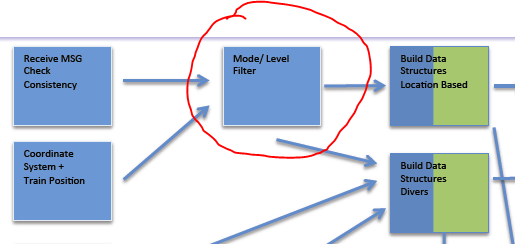
\includegraphics[scale=0.7]{images/FilterInandOUt}
\caption{Filter In and out}
\end{figure}

\subsubsection{SysML Model}
\begin{figure}[hbtp]
\centering
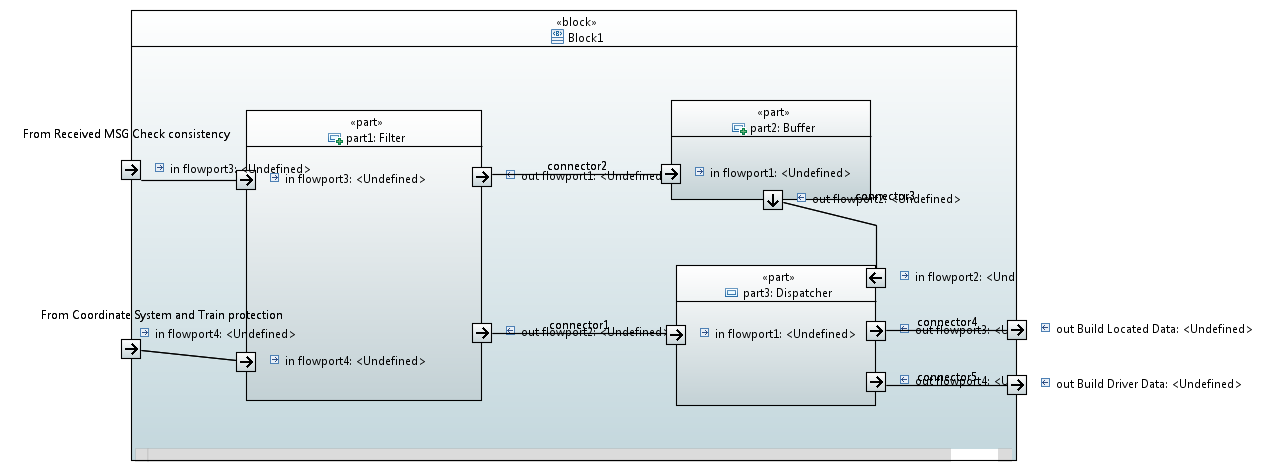
\includegraphics [scale=0.5]{images/SysMLFilter}
\caption{SysML Filter}
\end{figure}

\paragraph{Functional Design Description}
The fillter receives track information (balise an radio) and will filter them in dependency of the mode and level.
Therefore the filter needs the input from level and mode management. The filtered information will be forwarded to the data strcuture.

\begin{description}
\item[First filter] The first filter, i.e.~the filter on the level, is described in \cite[Chapter~4.8.3]{subset-026}.
\item[Second filter] The second filter, i.e.~the filter on the transition media, is described in\cite[Chapter~4.8.3]{subset-026}.
\item[Third filter]
 The third filter, i.e.~the filter on the modes, is described in \cite[Chapter~4.8.4]{subset-026}.
\item[Transition buffers] Details on the handling of the transition buffers used in the first and the second filter are described in \cite[Chapter~4.8.5]{subset-026}.
\end{description}

%%%% 
\subparagraph{Documentation of design}
From § 4.8.1.2 The following sections have to be interpreted by applying the filters and the assigned packets/messages as shown in Figure a and 2. The first filter is detailed in section § 4.8.3 (figure 1) “Accepted information depending on the level and transmission media”, the third filter in section § 4.8.4 (figure 2) “Accepted information depending on the modes”.\\

From § 4.8.1.3 If a message contains level transition information, any other information in that message shall be evaluated considering the level transition information. Explanation: If a message contains level transition information, all other information in that message shall be buffered and level transition shall be read first. Then the remained balise information shall be read from the buffer in the level that was announced to the balise.\\

From § 4.8.1.3.1 Information received in the same message as an immediate level transition order or a conditional level transition order that causes a level transition shall be evaluated first considering the on-board currently operated level, as if a level transition order for further location had been received (i.e. conditions [1], [2] or [6] of Figure 1, if applied, shall be automatically fulfilled). Then, if relevant, it shall be immediately extracted from the buffer and re-evaluated according to the new selected level.\\
\textbf{Explanation:} As described in Explanation of § 4.8.1.3 and figure 1 – First Filter conditions [1], [2] and [6])\\

From § 4.8.1.4 Note: As shown in Figure 1, information stored following an announcement of a change of level, is re-checked for acceptance when the level has changed. This implies that, when the level changes, the mode is - for a short moment – still unchanged, until the stored information has been processed. The consequence for the Third Filter is that information needs to be accepted for this short period also in modes in which this information is otherwise useless.\\
\textbf{Explanation:} when a level announced the level the mode change will be unchanged until the buffered information has been processed. The model change is the third filter (§ 4.8.3 figure 3).\\

\subparagraph{table for the filter rules}
\textbf{Assumptions from § 4.8.2 need to be considered}\\
\textbf{Explanation}: See figure 1 and 2 – announced packets/messages/variables to the filter. Exception and explanation of the meaning of R and A please read § 4.8.3.\\. 

\textbf {Filter rules}: Filter will filter messages, packages and variables. Therefole a rule must be defined to cover all these inputs.\\

\textbf {Explanation figure 1}: will filtering the different inputs in dependency of the level\\
\textbf {Explanation figure 2}: will filtering the different inputs in dependency of thel mode\\

\subparagraph{Filter on Level}
\begin{figure}[hbtp]
\centering
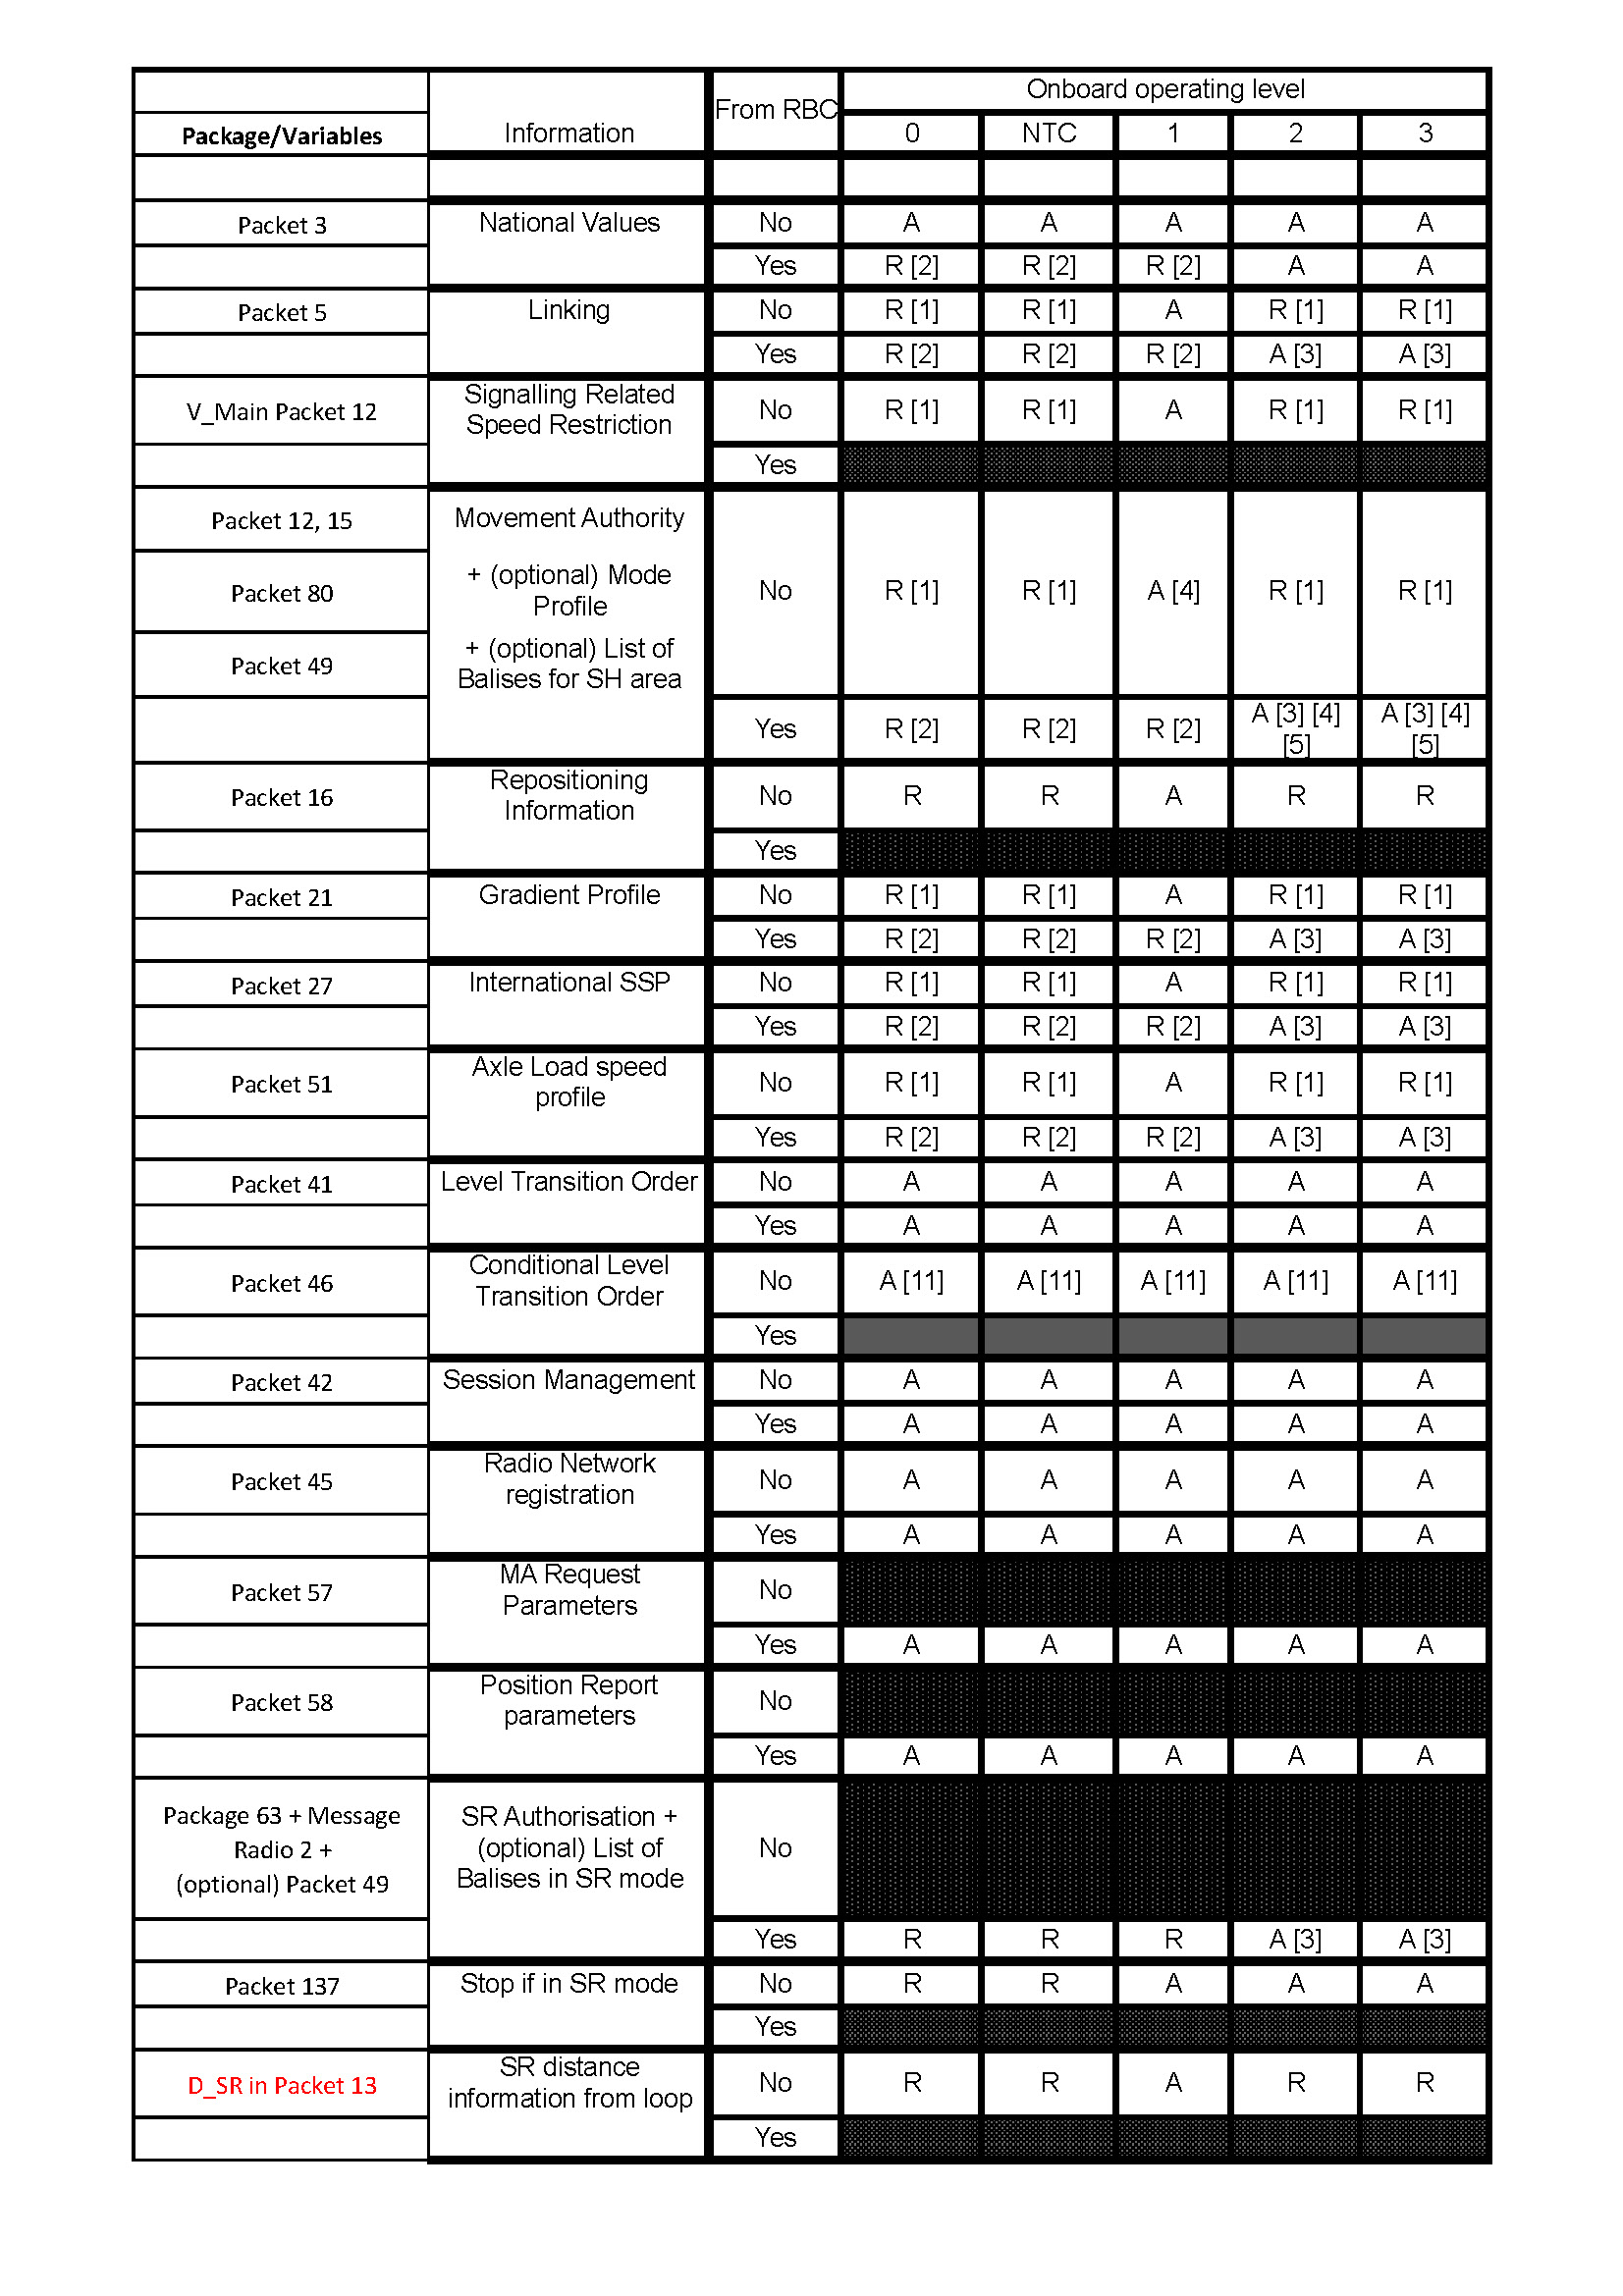
\includegraphics [scale=0.6]{images/LevelFilter1}
\end{figure}
\begin{figure}[hbtp]
\centering
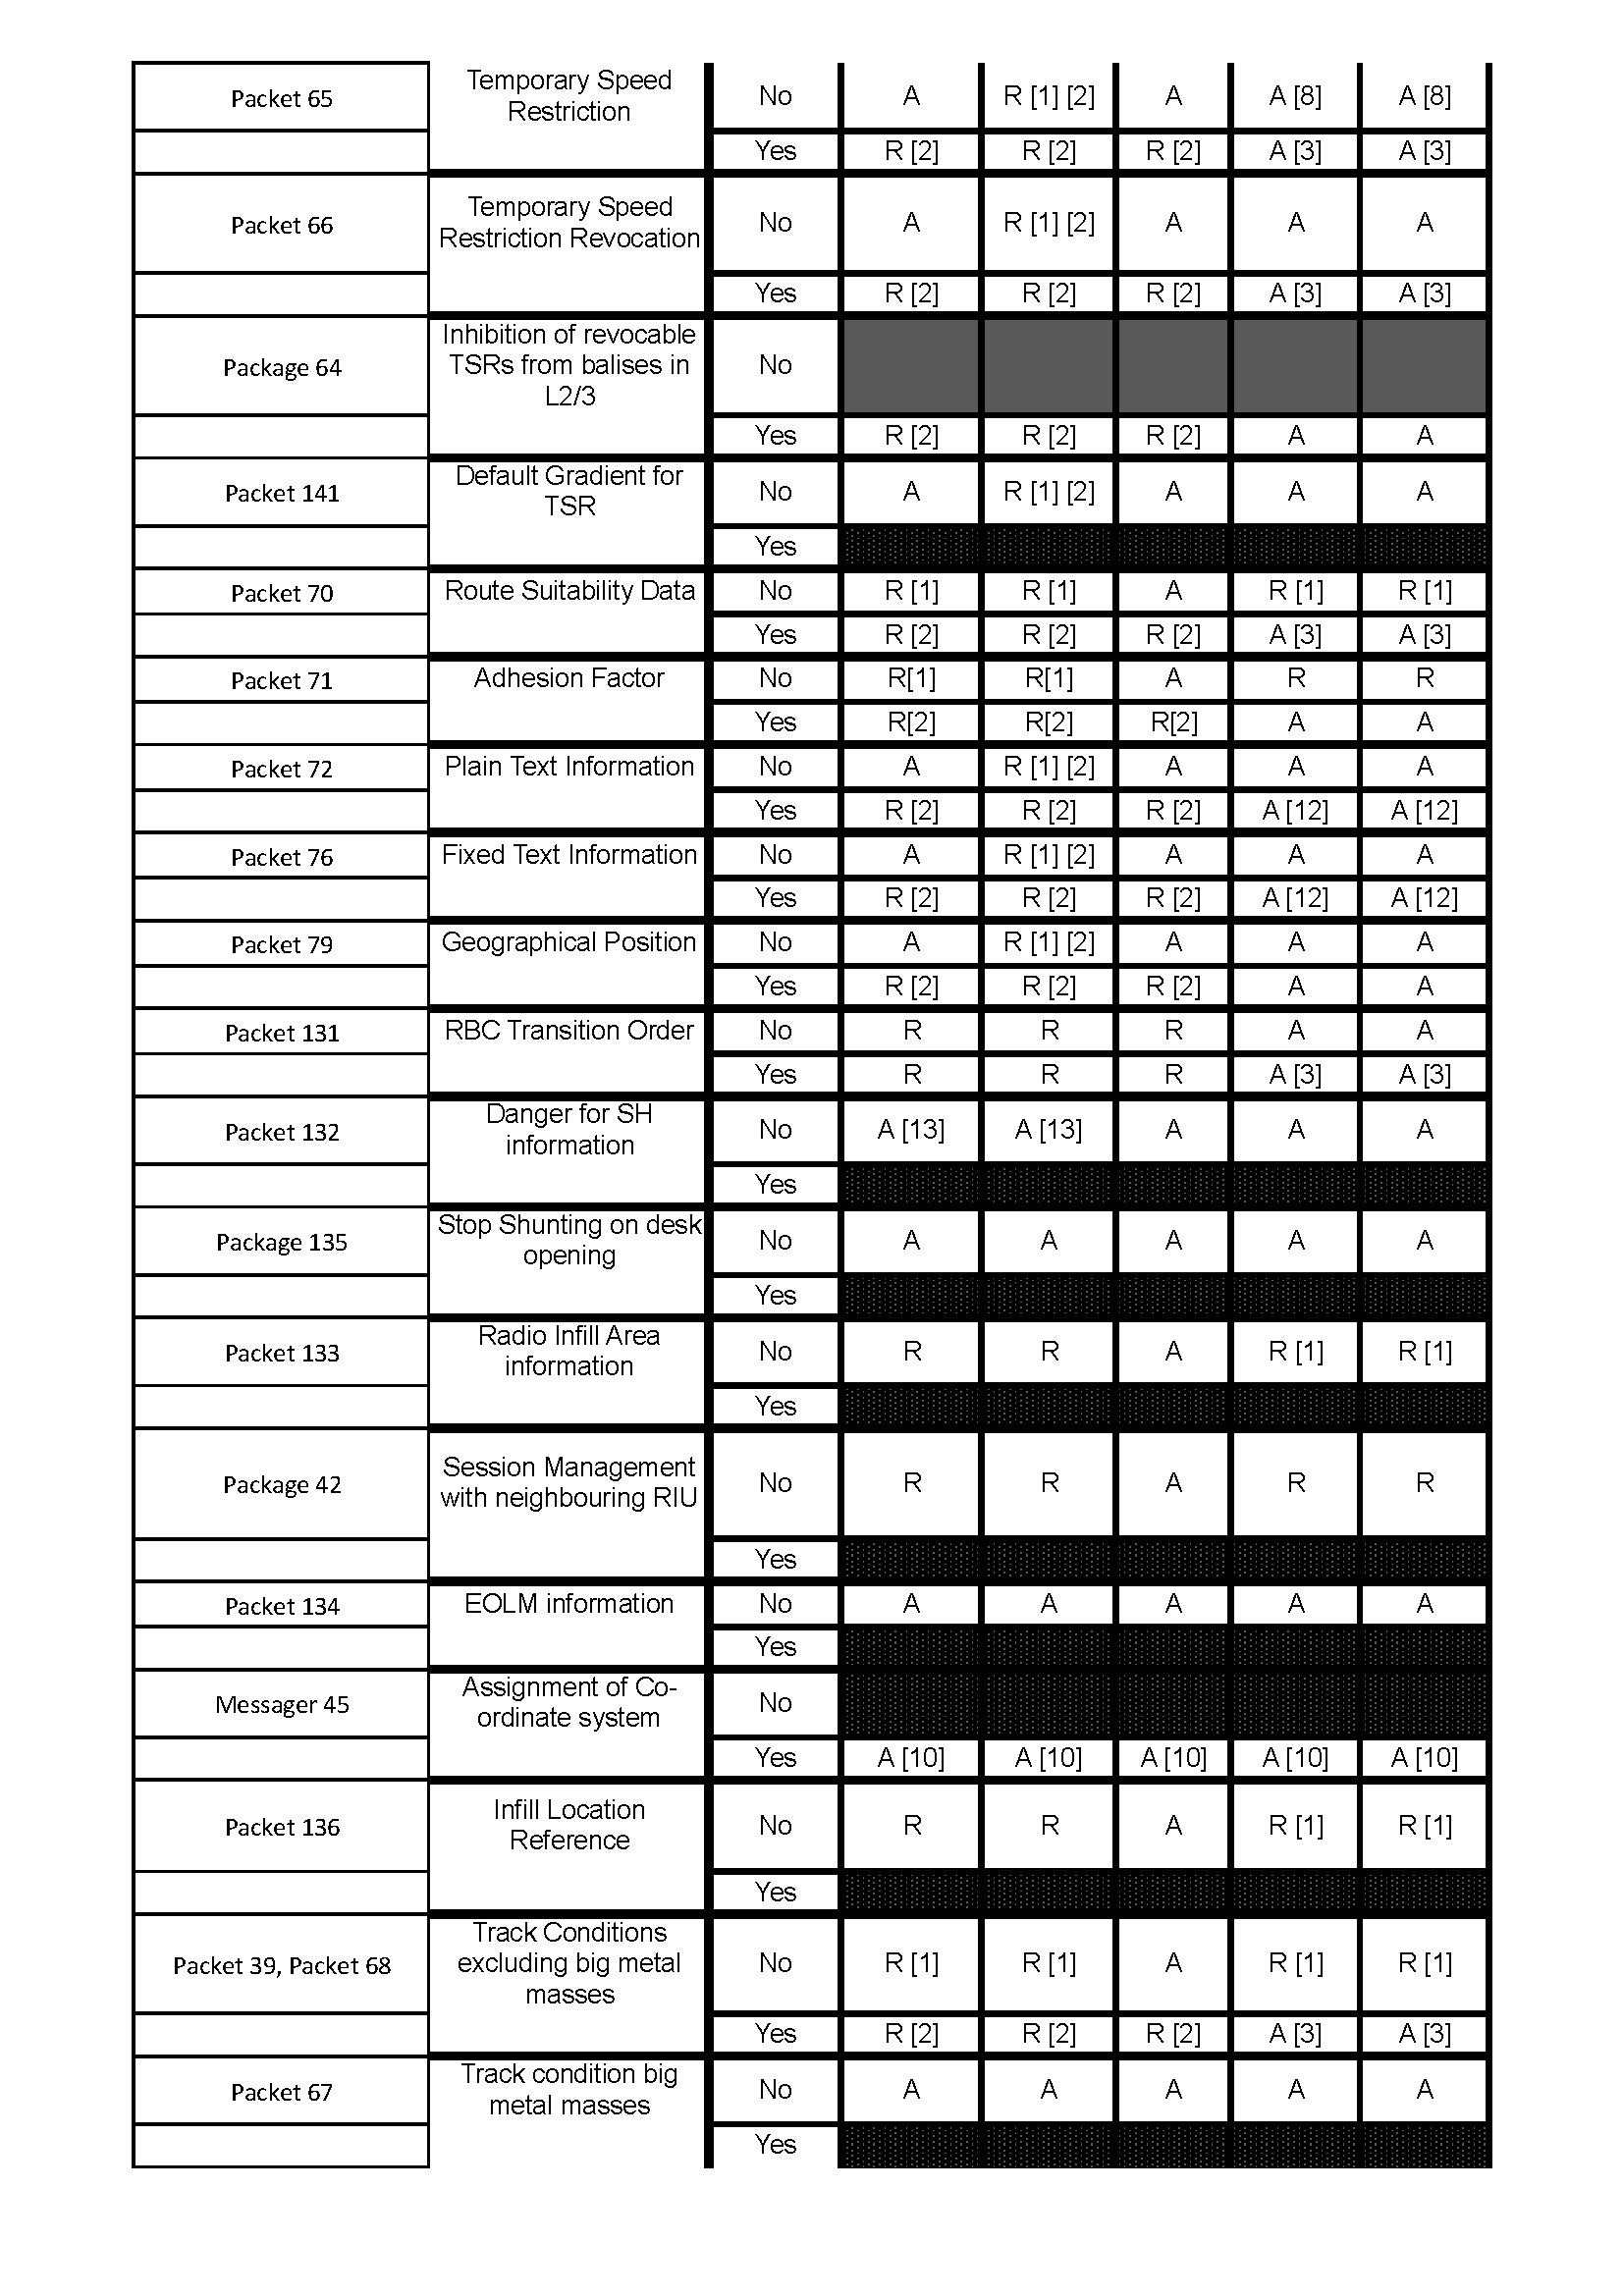
\includegraphics [scale=0.6]{images/LevelFilter2}
\end{figure}
\begin{figure}[hbtp]
\centering
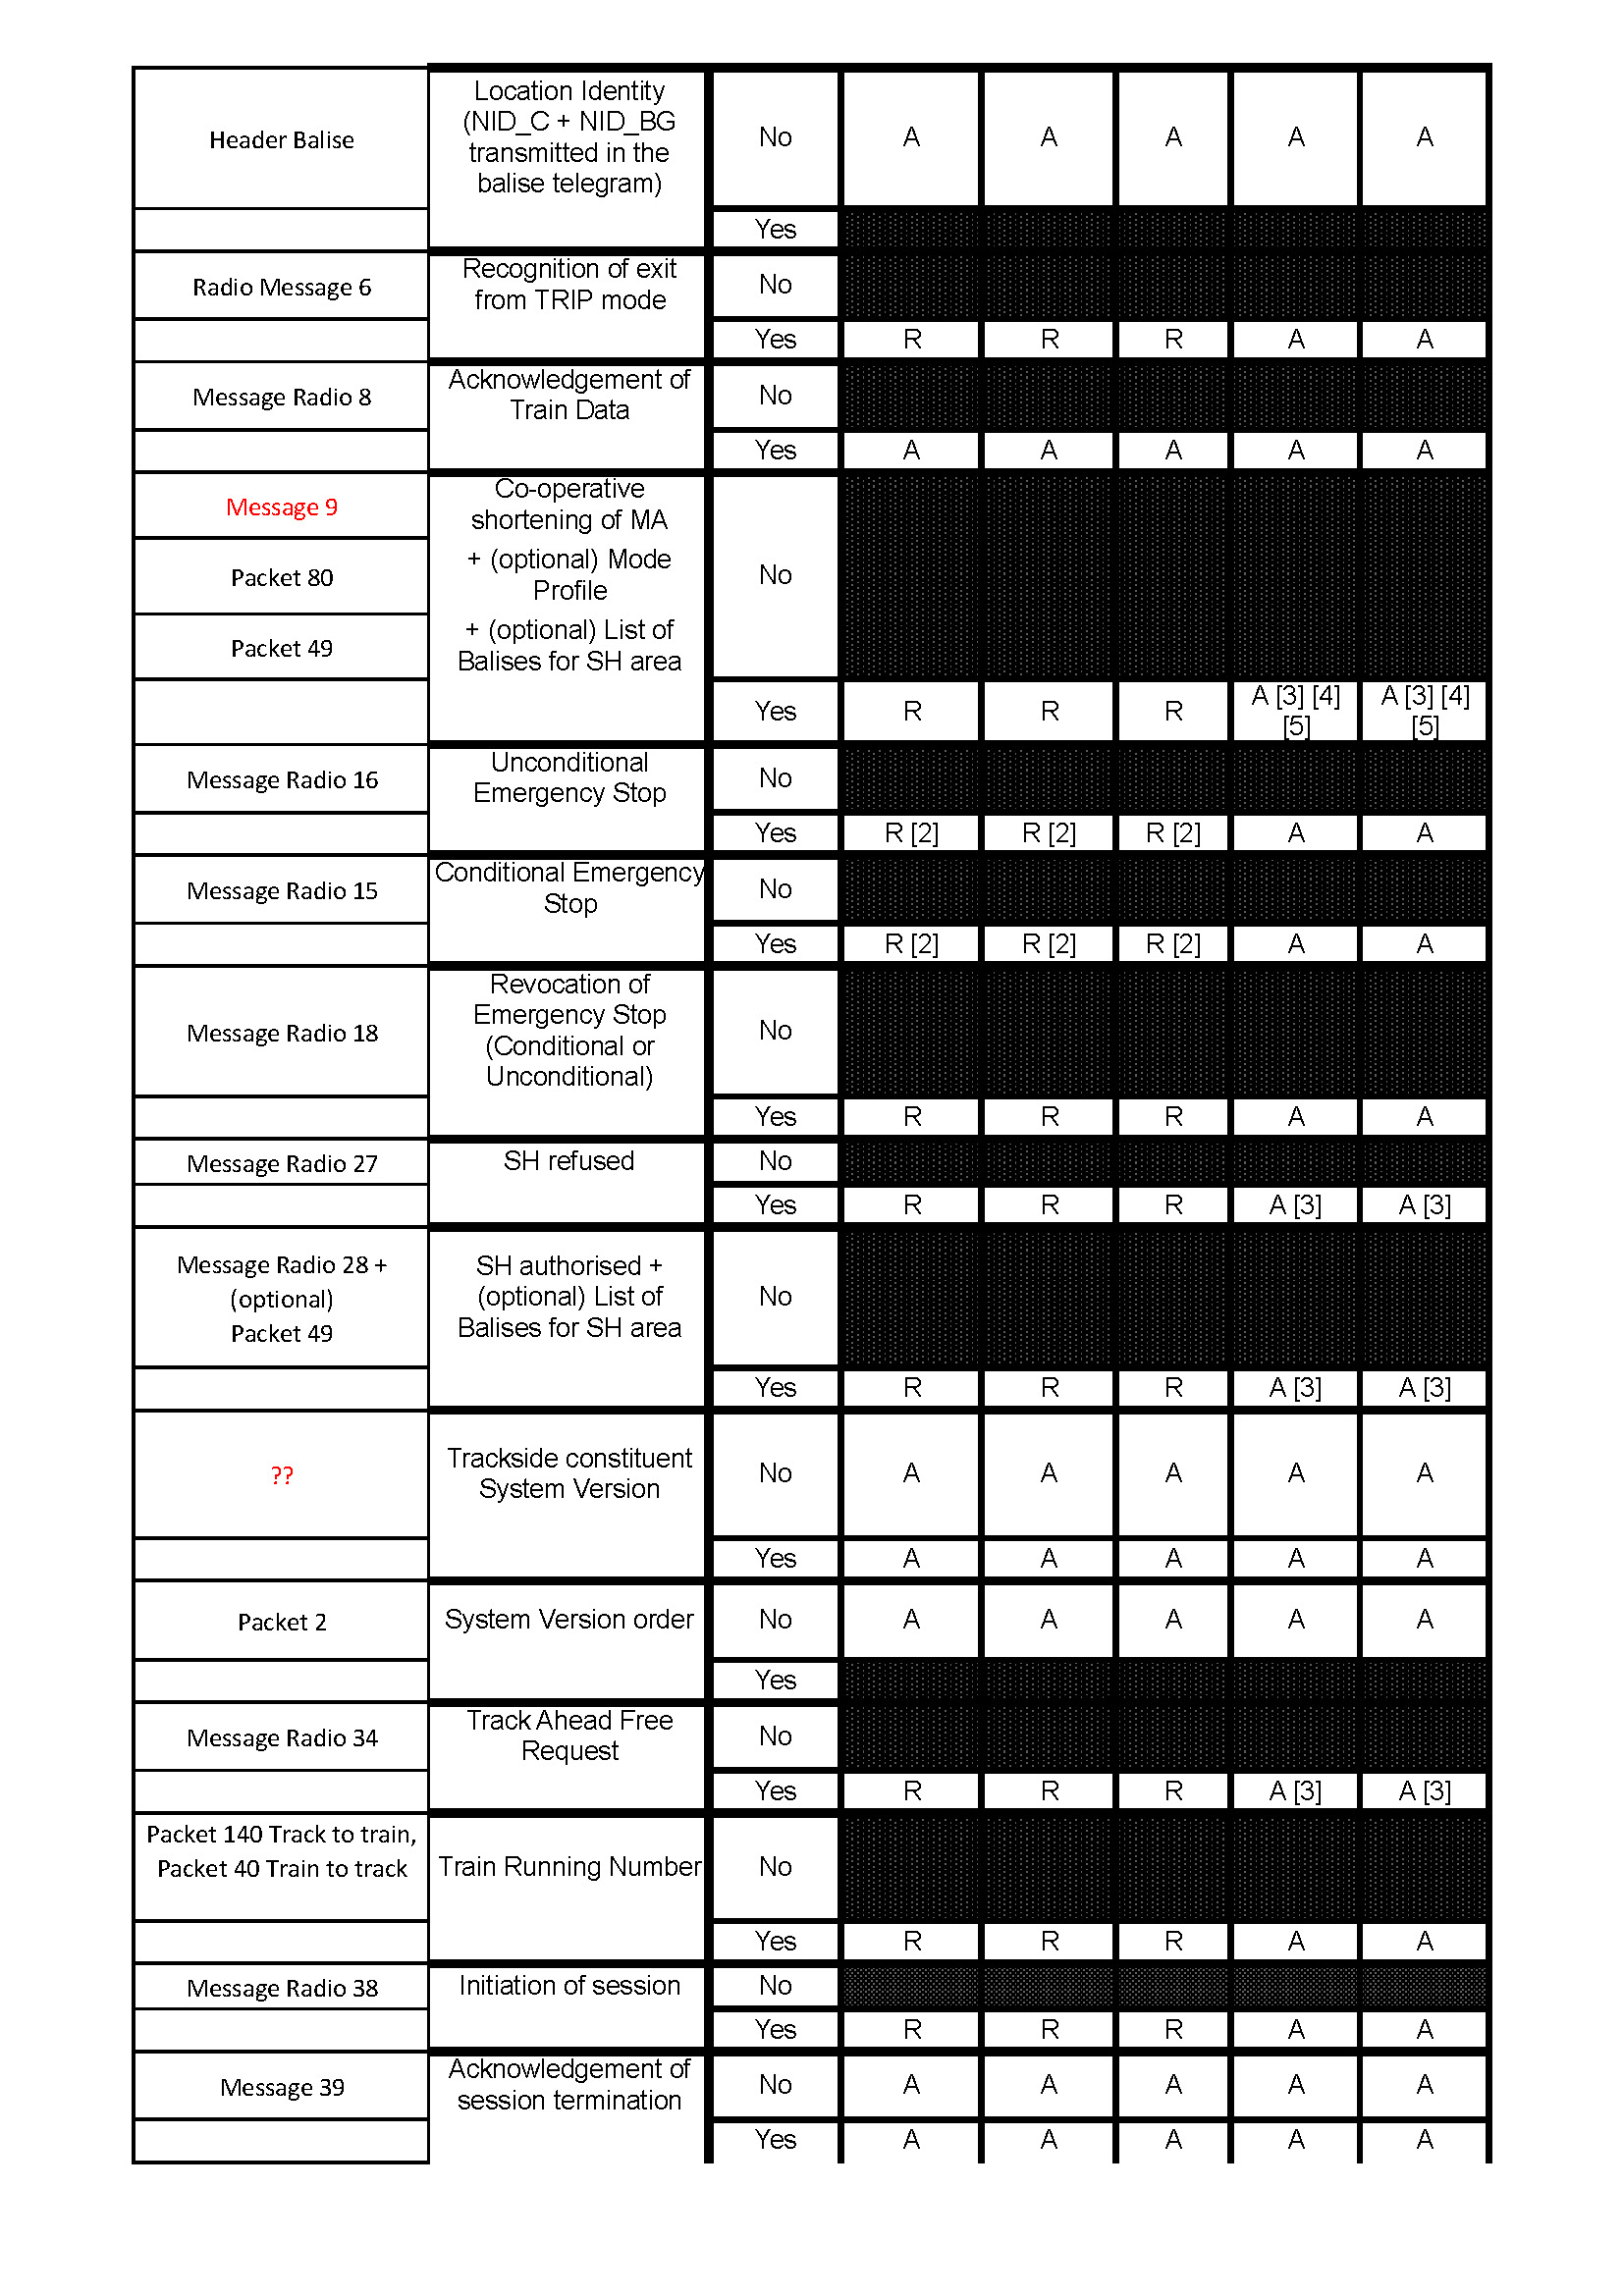
\includegraphics [scale=0.6]{images/LevelFilter3}
\end{figure}
\begin{figure}[hbtp]
\centering
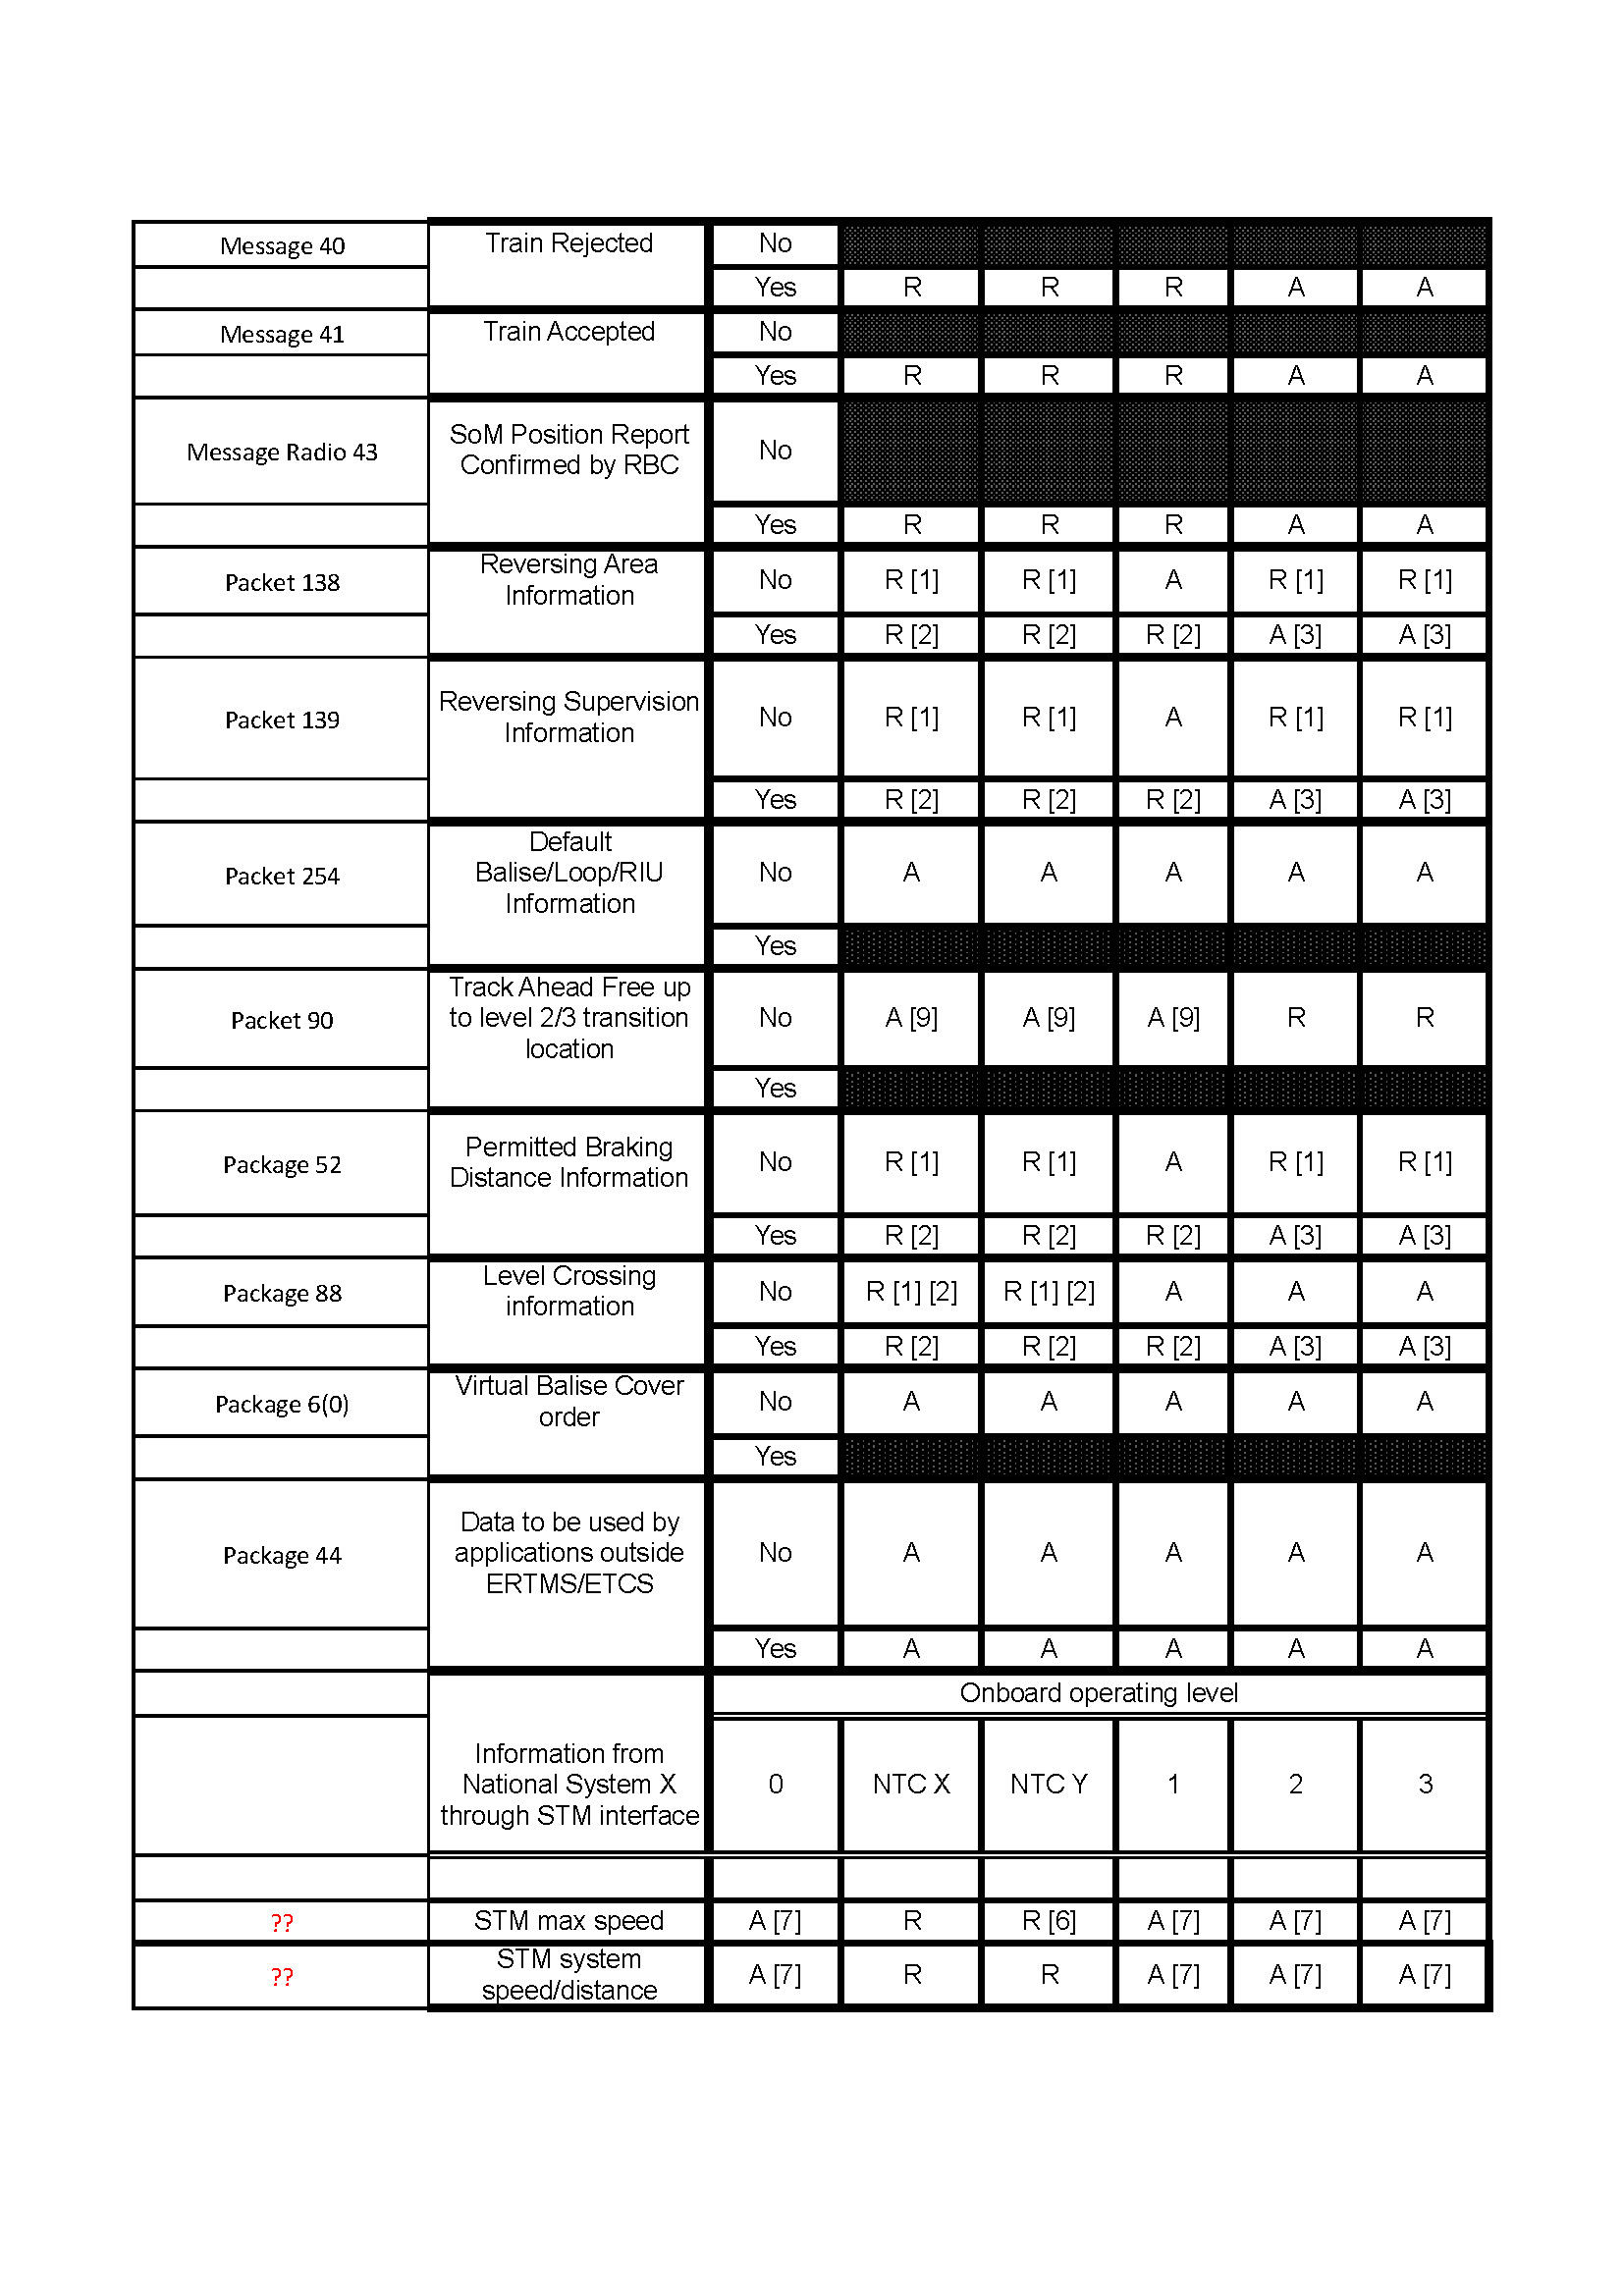
\includegraphics [scale=0.6]{images/LevelFilter4}
\caption{Level Filter}
\end{figure}
\newpage

\subparagraph{Filter on Modes}
\begin{figure}[hbtp]
\centering
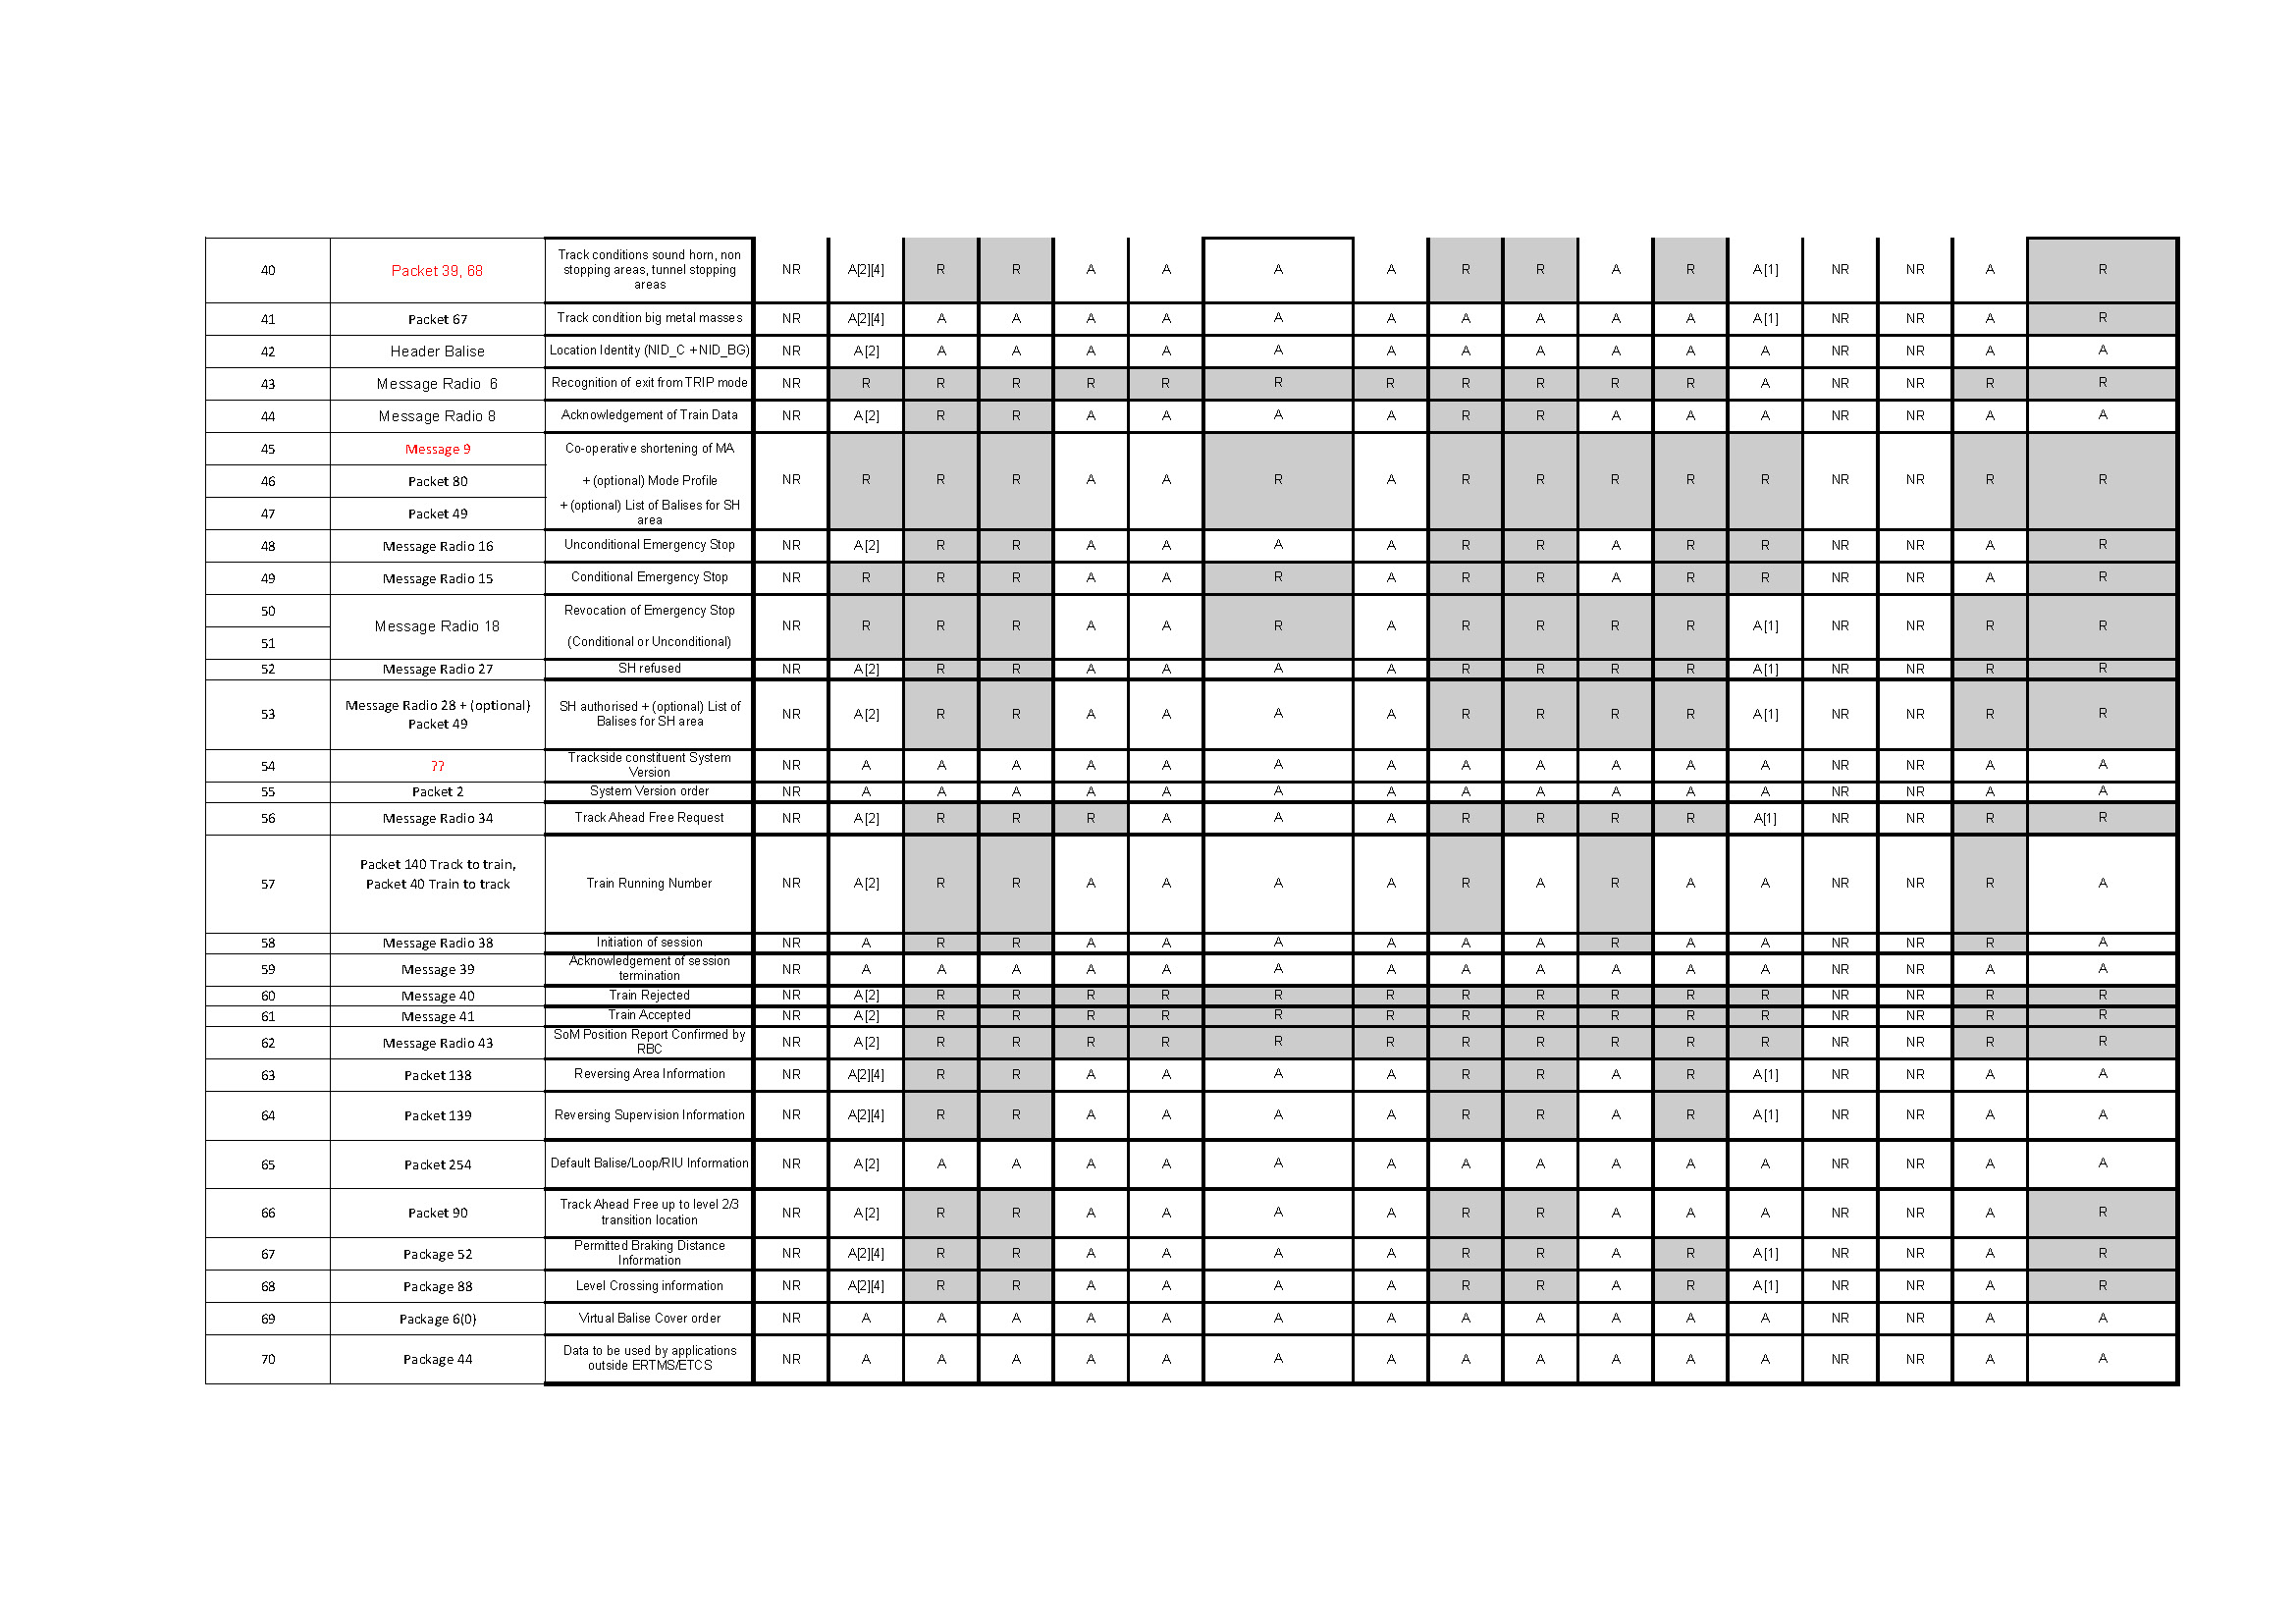
\includegraphics [angle=90, scale=0.8]{images/FilterMode1}
\end{figure}
\begin{figure}[hbtp]
\centering
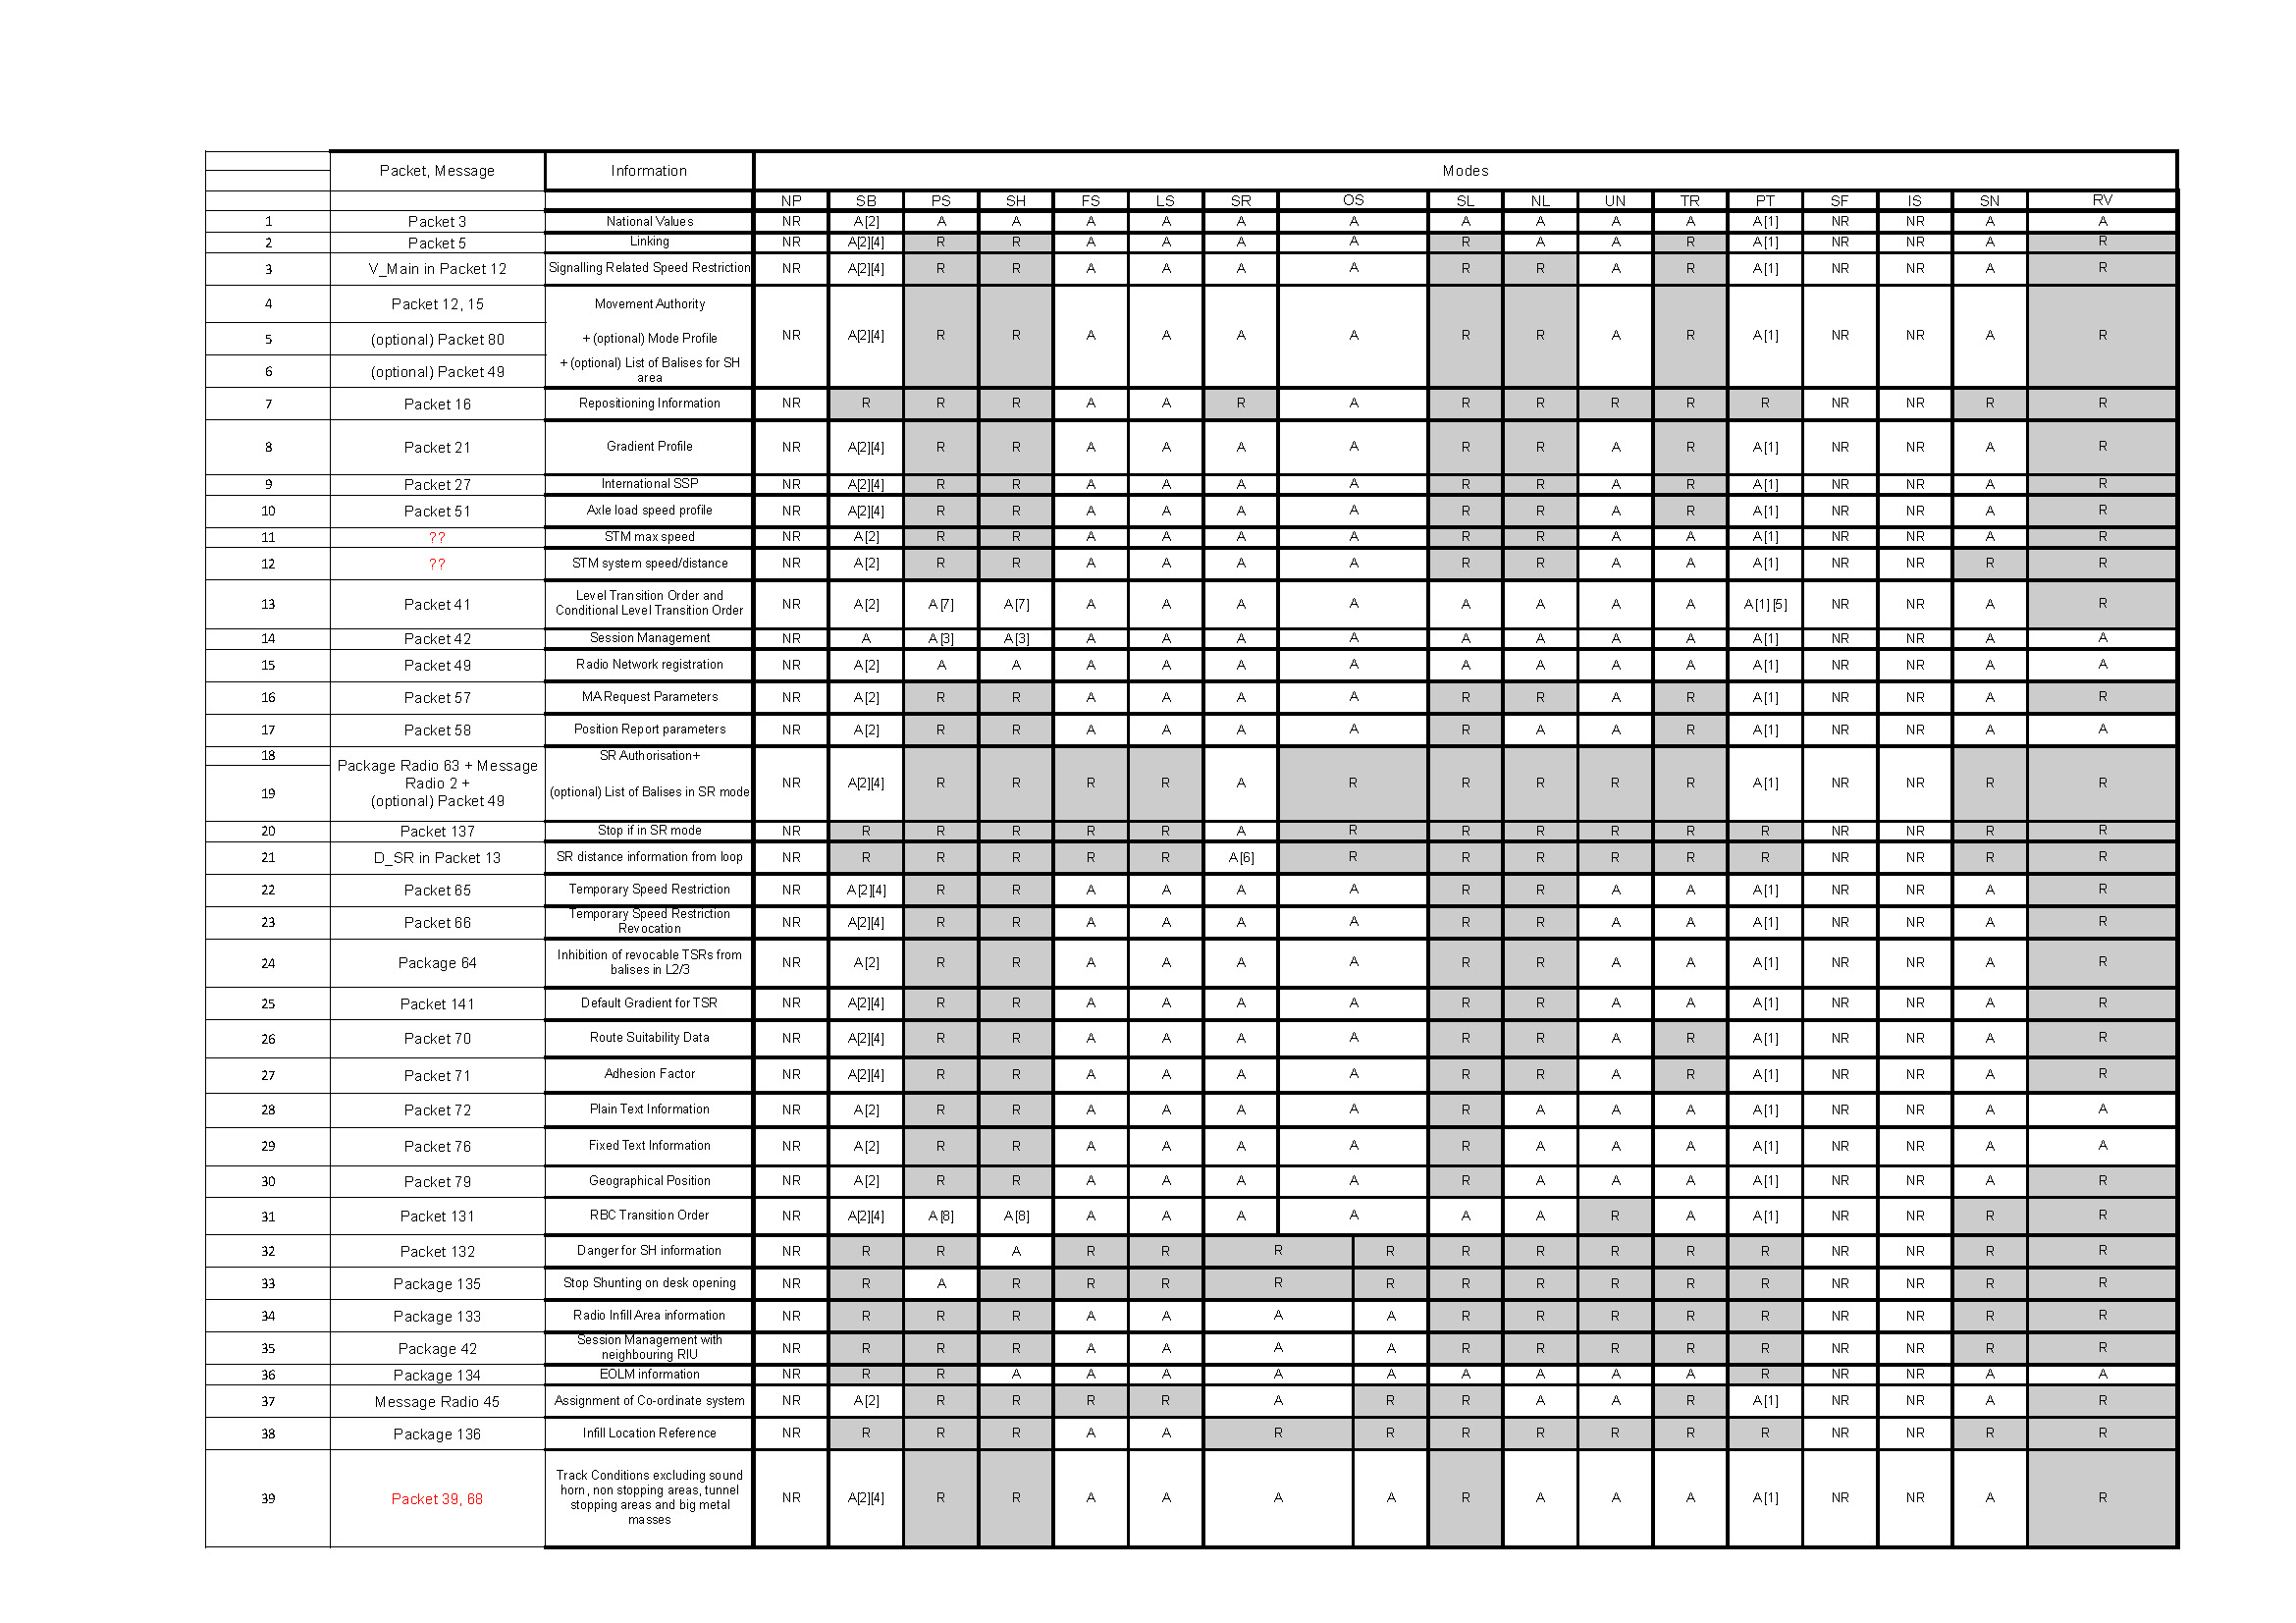
\includegraphics [angle=90, scale=0.8]{images/FilterMode2}
\end{figure}
\begin{figure}[hbtp]
\centering
\caption{Mode Filter}
\end{figure}
\newpage





\subparagraph{Filtering (Mode/Level) - One packet per type}
\textbf{ISSUE: HOW MANY PKT 44, 65 AND 66 PER MESSAGE ARE MAXIMALLY SUPPORTED? (BH: who made this comment??)}\\

- Check on announced and immediate level transition orders in the messages to be filtered (needed for further criteria for filtering, to decide if the data shall be stored in the transition buffer).\\
- Filter data stored in the transition buffer according to the current level (what to do if similar information is available in the new message??). Data can be rejected, accepted or kept in the transition buffer.
(Filtering according to new level will be done directly afterwards in the next cycle)\\
- Filter new received messages according to the current level (new level will be done in the next cycle as according to \gls{SRS} data first has to be filtered according to old level and afterwards to new level). Data can be rejected, accepted or stored in the transition buffer.\\
- Filter (level) accepted data according to originating RBC (supervising or other). Information from \gls{BG}'s, loops or RIU is not filtered with this filter.\\
- Filter (level and RBC) accepted data according to the current mode (only reject or accept)\\
\paragraph{Reference to the Scade Model}
\textbf{only in special case or link to the Scade model}